\documentclass[manuscript,review]{acmart}

%% Packages
\usepackage{graphicx}      
\usepackage{booktabs}        
\usepackage{multirow}        
\usepackage[ruled,vlined,linesnumbered]{algorithm2e} 
\usepackage{amsmath}        


\setcopyright{none}
\settopmatter{printacmref=false}
\renewcommand\footnotetextcopyrightpermission[1]{}



\captionsetup{justification=raggedright, singlelinecheck=false}


%% start
\begin{document}

\title{Between Lines of Code: Unraveling the Distinct Patterns of Machine and Human Programmers}

\author{Yuling Shi}
\affiliation{%
  \institution{Shanghai Jiao Tong University}
  \city{Shanghai}
  \country{China}}
\email{yuling.shi@sjtu.edu.cn}

\author{Hongyu Zhang}
\affiliation{%
  \institution{Chongqing University}
  \city{Chongqing}
  \country{China}}
\email{hyzhang@cqu.edu.cn}

\author{Chengcheng Wan}
\affiliation{%
  \institution{East China Normal University}
  \city{Shanghai}
  \country{China}}
\email{ccwan@sei.ecnu.edu.cn}

\author{Xiaodong Gu}
\affiliation{%
  \institution{Shanghai Jiao Tong University}
  \city{Shanghai}
  \country{China}}
\email{xiaodong.gu@sjtu.edu.cn}



%% abstract summary of paper
\begin{abstract}

The rapid evolution of large language models (LLMs) has transformed automated code generation, but it has also made it increasingly difficult to distinguish between human-written and machine-generated code. This ambiguity creates practical challenges for software integrity, code ownership, and security. While zero-shot detection tools like DetectGPT work well for natural language, they struggle with source code due to its strict syntactic rules. This paper reproduction summarizes the work of Shi et al., who conducted an empirical analysis comparing the stylistic differences between human and AI programmers. Their findings indicate that machine-generated code is typically more concise, uses a narrower vocabulary, and is highly predictable—particularly regarding the placement of whitespace and newlines. Based on these insights, the original authors developed DetectCodeGPT, a zero-shot detection framework that perturbs code by inserting random spaces and newlines rather than altering structural tokens. The reproduced evaluation demonstrates that this stylized perturbation approach outperforms existing baselines in identifying machine-generated code across multiple LLMs, without requiring an external perturbation model.

\end{abstract}

\maketitle


%%  sections mentioned
\section{Introduction}
\label{sec:intro}

The rise of large language models (LLMs) such as Codex~\cite{chen2021evaluating} and ChatGPT~\cite{openai2022chatgpt} has changed how software is written. Trained on enormous code corpora scraped from open-source repositories, these models can now produce code that is often syntactically correct and functionally reasonable, and they are increasingly used throughout the software development lifecycle~\cite{roziere2023codellama}.

This convenience comes with a cost: it is no longer obvious whether a given piece of code was written by a human or generated by a model. Shi et al.~\cite{shi2024between} point out that this ambiguity is not a merely academic concern. It complicates bug triage and code-ownership attribution, it can inflate assessments of a developer's productivity, and it allows latent vulnerabilities to go unnoticed because reviewers over-trust code that ``looks'' machine-produced and therefore assume it is robust. More broadly, when the provenance of code is unclear, the transparency of the entire development process is put at risk.

A natural place to look for a solution is the literature on detecting machine-generated \emph{text}. Zero-shot, perturbation-based detectors such as DetectGPT~\cite{mitchell2023detectgpt} have become the state of the art for that problem: they exploit the fact that machine-generated text tends to sit at a sharper local maximum of the model's likelihood function, so that small perturbations of the text cause a larger drop in log-probability than similar perturbations do for human-written text. The trouble is that this idea was designed for natural language, which tolerates a great deal of lexical and syntactic variation. Source code does not: it must obey a rigid grammar in order to even parse, let alone execute. As the original authors argue, this mismatch means that natural-language detectors transfer poorly to code, and it is exactly why a systematic study of \emph{what actually distinguishes} machine- and human-authored code was still missing before this work.

This study addresses that gap directly by conducting a controlled empirical comparison of human- and machine-authored Python functions along three axes -- lexical diversity, conciseness, and naturalness -- and show that machine-generated code is measurably more concise and more ``natural'' (i.e., more predictable under a language model) than human code, that it draws from a narrower vocabulary, and that it still follows familiar programming idioms. Crucially, they find that this gap is largest not in ordinary tokens but in \emph{stylistic} tokens: whitespace and newlines. Building on that observation, they propose \textbf{DetectCodeGPT}, a perturbation-based detector that -- instead of calling out to an external masked-language model to rewrite tokens, as DetectGPT does -- perturbs code directly by inserting spaces and newlines at randomly chosen positions. This removes the dependency on a second, external model and makes the method considerably cheaper to run while, according to the paper, also making it more effective.

Across two datasets and six open code LLMs ranging from 1.3B to 7B parameters, DetectCodeGPT is reported to outperform the strongest prior baseline by an average of 7.6\% in AUROC, and it degrades only mildly when the model used for detection differs from the model that actually generated the code -- an important property for real-world deployment, where the source model is rarely known.

The main contributions of this paper are threefold: (1) a systematic empirical study of the stylistic differences between LLM-generated and human-written code; (2) a new detection method, DetectCodeGPT, that exploits those differences through a stylized, model-free perturbation strategy; and (3) an extensive evaluation of that method across models, datasets, and ablations.

The remainder of this summary is organized as follows. Section~\ref{sec:background} covers the background on code LLMs and on perturbation-based text detection that motivates the paper. Section~\ref{sec:method} describes the empirical study design and the DetectCodeGPT algorithm itself. Section~\ref{sec:results} reports the empirical findings and the detection performance results. Section~\ref{sec:discussion} discusses why the method works, its limitations, and closes with a short reflection.

\section{Background and Related Work}
\label{sec:background}

\subsection{Large Language Models for Code}
Modern code LLMs are, almost without exception, decoder-only Transformers~\cite{vaswani2017attention} trained on very large text corpora. Codex~\cite{chen2021evaluating} and AlphaCode were among the first to show that this recipe, applied to millions of GitHub repositories, produces models capable of writing functionally correct code from a natural-language description. Follow-up work improved on this basic recipe along two main lines: new pretraining objectives such as fill-in-the-middle, which teach a model to complete code given both a prefix and a suffix, and instruction fine-tuning, which aligns a model's outputs with what a user actually asks for. More recent general-purpose models such as ChatGPT and LLaMA are trained on a mixture of natural language and code and perform well on code generation despite not being code-specialized. Code Llama~\cite{roziere2023codellama}, the model family used as the code generator in the reproduced study, is one such model, further specialized for code through continued pretraining on code-heavy data.

\subsection{Perturbation-Based Detection of Machine-Generated Text}
This work builds directly on DetectGPT~\cite{mitchell2023detectgpt}, adapting its core idea for code. DetectGPT assumes access to the log-probability function $\log p_\theta(\cdot)$ of the (candidate) source model. Given a passage $x$, it draws a set of small perturbations $\tilde{x} \sim q(\cdot\,|\,x)$ -- originally, by masking spans of $x$ and having a separate model such as T5 fill them back in -- and computes the discrepancy
\begin{equation}
d(x, p_\theta, q) \triangleq \log p_\theta(x) - \mathbb{E}_{\tilde{x}\sim q(\cdot|x)}\big[\log p_\theta(\tilde{x})\big].
\label{eq:detectgpt}
\end{equation}
The intuition is that machine-generated passages sit near a local maximum of $\log p_\theta$: because the model wrote them, they are close to what the model considers highly probable, so any small rewriting tends to \emph{lower} their probability noticeably, producing a large, positive value of $d$. Human-written passages, in contrast, reflect a far more varied distribution of experience and phrasing, so they are less tightly bound to any single model's notion of what is likely, and $d$ tends to stay small. A sufficiently large $d(x,p_\theta,q)$ is therefore taken as evidence of machine authorship.

This idea is elegant for natural language, but it leans on an assumption that does not hold for code: that a random local rewrite of $x$ is still a coherent, ``in-distribution'' example of the same kind of content. Natural language tolerates this -- a masked-and-refilled sentence is usually still grammatical. Code frequently does not: masking and refilling a token can turn a valid program into one that no longer parses, changing $\log p_\theta$ for reasons that have nothing to do with authorship. This is precisely the gap that motivates the empirical study in Section~\ref{sec:method} and the subsequent perturbation strategy in Section~\ref{sec:method-detect}.

\subsection{Related Detection Methods}
Work on detecting machine-generated \emph{text} broadly falls into two families: zero-shot methods, which use likelihood or rank statistics directly (as DetectGPT and its NPR-based successor DetectLLM~\cite{su2023detectllm} do) and require no labeled data, and supervised methods, which fine-tune a classifier such as RoBERTa on generations collected from specific model families. Zero-shot methods generalize better to unseen source models but are typically more computationally expensive per example, since most of them call an auxiliary model to generate perturbations.

Work specifically on machine-generated \emph{code} detection is comparatively sparse. GPTSniffer~\cite{nguyen2023snippet} is a supervised baseline that fine-tunes CodeBERT to classify a snippet's authorship; DetectCodeGPT outperforms this supervised baseline on average, which is notable since GPTSniffer has the advantage of having seen labeled training examples. A separate line of work, code watermarking~\cite{lee2023watermarking}, takes an entirely different approach: rather than detecting authorship after the fact, it embeds an imperceptible marker into generated code during training or decoding. Watermarking can be very reliable when applicable, but it requires cooperation from whoever controls the generating model, which makes it unsuitable for the more general, model-agnostic detection setting that DetectCodeGPT targets.

\section{Method}
\label{sec:method}

The methodology consists of two main parts. First, an empirical study is used to characterize how human- and machine-authored code differ along three dimensions. Second, these findings are translated into a concrete detection algorithm called DetectCodeGPT.

\subsection{Empirical Study Design}
\label{sec:study-design}
The authors organize their comparison around three properties commonly used to describe coding style: \emph{lexical diversity}, \emph{conciseness}, and \emph{naturalness}.

\textbf{Lexical diversity} is assessed with four metrics. \emph{Token frequency} simply counts how often each distinct token occurs. \emph{Syntax element distribution} groups tokens into seven coarse categories using the \texttt{tree-sitter} parser, reproduced in Table~\ref{tab:categories}, and compares the proportion of each category between the two sources. \emph{Zipf's law}, which states that a token's frequency is roughly inversely proportional to its frequency rank, and \emph{Heaps' law}, which describes how the size of a corpus's vocabulary grows with corpus length, are both checked for machine- and human-written code to see whether machine code follows the same statistical regularities as human code, and how quickly its vocabulary grows.

%% @{} & midrule toprule syntax 
\begin{table}[t]
\caption{Studied categories of Python code tokens, as classified by the \texttt{tree-sitter} parser.}
\label{tab:categories}
\begin{tabular}{@{}ll@{}}
\toprule
\textbf{Category} & \textbf{Example tree-sitter types} \\
\midrule
keyword          & \texttt{def}, \texttt{return}, \texttt{else}, \texttt{if}, \texttt{for}, \ldots \\
identifier       & \texttt{identifier}, \texttt{type\_identifier} \\
literal          & \texttt{string\_content}, \texttt{integer}, \texttt{true}, \ldots \\
operator         & \texttt{<}, \texttt{>}, \texttt{=}, \texttt{==}, \texttt{+}, \ldots \\
syntactic symbol & \texttt{:}\, \texttt{)}\, \texttt{]}\, \texttt{[}\, \texttt{(}\, \texttt{,}\, \texttt{"}\, \texttt{\{}\, \texttt{\}}\, \texttt{.} \\
comment          & \texttt{comment} \\
whitespace       & space, newline \\
\bottomrule
\end{tabular}
\end{table}

\textbf{Conciseness} is measured simply by the number of tokens and the number of lines in a snippet, which together capture both raw verbosity and how a developer chooses to lay code out across lines.

\textbf{Naturalness}, following the ``naturalness of software'' hypothesis~\cite{hindle2016naturalness} that programs are, statistically, at least as regular and predictable as natural language, is quantified with two per-token statistics under a language model $p_\theta$: the \emph{log likelihood} $\log p_\theta(x)$ of a token, and its \emph{log rank} $\log r_\theta(x)$, i.e., the log-position of the token in the list of all vocabulary tokens sorted by the model's predicted probability at that position. Lower rank and higher likelihood both indicate a token the model considers highly predictable, i.e., more ``natural.''

\subsection{Dataset and Experimental Setup for the Empirical Study}
Human-authored code is drawn from 10{,}000 Python functions sampled from CodeSearchNet~\cite{husain2020codesearchnet}, a corpus of real-world functions scraped from open-source GitHub projects. For each function, its signature and docstring are used as a prompt to Code Llama-7B~\cite{roziere2023codellama}, and the model's completion is treated as the ``machine-authored'' counterpart to that same function's human-written body. Generation uses top-$p$ (nucleus) sampling~\cite{holtzman2019curious} with $p=0.95$ at two temperatures, $T=0.2$ and $T=1.0$, capturing both a conservative and an exploratory generation regime, with completions capped at 512 tokens.

The choice of CodeSearchNet over curated benchmarks such as HumanEval is deliberate: HumanEval-style problems are short, self-contained programming exercises, whereas CodeSearchNet functions come from real production codebases with the messiness -- and the individual style -- that entails. This makes the comparison more representative of how machine- and human-written code actually differ ``in the wild,'' at some cost to how well the model performs on any single function.

\subsection{The DetectCodeGPT Algorithm}
\label{sec:method-detect}
The empirical results (detailed in Section~\ref{sec:results}) show that the naturalness gap between machine- and human-written code is largest specifically in whitespace tokens. DetectCodeGPT turns this observation into a perturbation strategy: rather than perturbing arbitrary tokens with an external masked-language model, it perturbs only whitespace, directly and cheaply.

\textbf{Problem formulation.} Detection is framed as classifying whether a snippet $x$ was produced by a source model $p_\theta$. As in DetectGPT, this is done by perturbing $x$ into $\tilde{x} \sim q(\cdot\,|\,x)$ and looking for a sharp change in a naturalness score.

\textbf{Naturalness score.} Instead of the raw log-likelihood gap of Equation~\ref{eq:detectgpt}, DetectCodeGPT adopts the Normalized Perturbed Log Rank (NPR) score, which prior work on text detection found to be smoother and more robust than a likelihood-based score:
\begin{equation}
\mathrm{NPR}(x, p_\theta, q) \triangleq \frac{\mathbb{E}_{\tilde{x}\sim q(\cdot|x)}\big[\log r_\theta(\tilde{x})\big]}{\log r_\theta(x)}.
\label{eq:npr}
\end{equation}
Intuitively, if perturbing $x$ causes its average token rank to worsen by a lot relative to its own original rank, $x$ is more likely to be machine-authored.

\textbf{Perturbation strategy.} Two lightweight, purely syntactic perturbations are used, chosen independently at random for each of $k$ perturbed samples:
\begin{itemize}
  \item \emph{Space insertion.} Let $C$ be the set of all candidate positions where a space could be inserted in $x$. A random subset $C_s \subseteq C$ of size $\alpha|C|$ is chosen, and at each chosen position $c$, a number of spaces
  \begin{equation}
    n_{\text{spaces}}(c) \sim \mathrm{Poisson}(\lambda_{\text{spaces}})
    \label{eq:spaces}
  \end{equation}
  is inserted.
  \item \emph{Newline insertion.} Symmetrically, $x$ is split into lines $L$, a random subset $L_n \subseteq L$ of size $\beta|L|$ is chosen, and after each chosen line $l$, a number of newlines
  \begin{equation}
    n_{\text{newlines}}(l) \sim \mathrm{Poisson}(\lambda_{\text{newlines}})
    \label{eq:newlines}
  \end{equation}
  is inserted.
\end{itemize}
Sampling the insertion counts from a Poisson distribution -- rather than always inserting a fixed amount -- is meant to imitate the irregular, unplanned way a human tends to space out their code, which is exactly the kind of variation Finding~5 in Section~\ref{sec:results} shows is missing from machine-generated whitespace.

Because both perturbations only ever \emph{add} whitespace, they cannot change the tokenization of the surrounding code or break its syntax -- unlike DetectGPT's mask-and-refill perturbation, which can silently turn valid code into invalid code and corrupt the very signal the detector relies on.

\textbf{Decision rule.} Algorithm~\ref{alg:detectcodegpt} summarizes the full procedure. The final score is the NPR of the original snippet minus the average NPR of its $k$ perturbed variants; a score above a threshold $\epsilon$ is classified as machine-authored.



%% algorithm 
\begin{algorithm}[t]
\caption{DetectCodeGPT: machine-generated code detection via stylized code perturbation}
\label{alg:detectcodegpt}
\KwIn{code $x$; source model $M$; number of perturbations $k$; decision threshold $\epsilon$; hyperparameters $\alpha,\beta,\lambda_{\text{spaces}},\lambda_{\text{newlines}}$}
\KwOut{\textbf{true} if $x$ is probably machine-authored, \textbf{false} otherwise}
\For{$i \leftarrow 1$ \KwTo $k$}{
  draw $p \sim \mathrm{Uniform}(0,1)$\;
  \eIf{$p \le 0.5$}{
    \tcp{space insertion}
    let $C$ = all candidate positions to insert a space in $x$\;
    sample $C_s \subseteq C$ with $|C_s| = \alpha|C|$\;
    \ForEach{position $c \in C_s$}{
      $n_{\text{spaces}}(c) \sim \mathrm{Poisson}(\lambda_{\text{spaces}})$\;
      insert $n_{\text{spaces}}(c)$ spaces at $c$\;
    }
  }{
    \tcp{newline insertion}
    split $x$ into lines $L$\;
    sample $L_n \subseteq L$ with $|L_n| = \beta|L|$\;
    \ForEach{line $l \in L_n$}{
      $n_{\text{newlines}}(l) \sim \mathrm{Poisson}(\lambda_{\text{newlines}})$\;
      insert $n_{\text{newlines}}(l)$ newlines after $l$\;
    }
  }
  store the perturbed code as $\tilde{x}_i$\;
}
$\displaystyle \mathrm{NPR}_x \leftarrow \mathrm{NPR}(x,p_\theta,q) - \frac{1}{k}\sum_{i=1}^{k} \mathrm{NPR}(\tilde{x}_i,p_\theta,q)$\;
\eIf{$\mathrm{NPR}_x > \epsilon$}{
  \Return{\textbf{true}} \tcp*{probably machine-authored}
}{
  \Return{\textbf{false}} \tcp*{probably human-authored}
}
\end{algorithm}


The threshold $\epsilon$ trades off false positives against false negatives and can be tuned per deployment; all evaluation in Section~\ref{sec:results} instead reports threshold-independent AUROC.



\section{Findings and Results}
\label{sec:results}

This section details two primary sets of results: the empirical patterns that distinguish human- from machine-authored code, and the detection performance of the DetectCodeGPT algorithm.

\subsection{Patterns That Distinguish Human and Machine Code}

\textbf{Token frequency.} Looking at the most frequent tokens in each corpus, both sources share the expected backbone of any Python program -- punctuation like \texttt{.}, \texttt{(}, \texttt{)}, and control-flow keywords like \texttt{if}, \texttt{return}, \texttt{else} -- which is unsurprising since the model itself was trained on human code and inherits its basic syntax. The more interesting gap is in exception-handling and object-oriented vocabulary: tokens such as \texttt{raise}, \texttt{TypeError}, and \texttt{isinstance} are noticeably more frequent in machine output, as are boilerplate identifiers like \texttt{\_\_class\_\_} and \texttt{\_\_name\_\_}. This suggests machine-generated code leans more heavily, and more explicitly, on defensive programming and object-oriented conventions than the human baseline does.

\begin{quote}
\textit{Finding 1.} Machine-authored code shows more attention to exception handling and object-oriented idiom than human code, consistent with an emphasis on error prevention and adherence to common programming paradigms.
\end{quote}

\textbf{Syntax element distribution.} Figure~\ref{fig:syntax-dist} breaks tokens down into the seven categories of Table~\ref{tab:categories} and compares their proportions between sources at both temperatures. Keyword, operator, symbol, and whitespace proportions are nearly identical between human and machine code, which the authors read as evidence that the foundational grammar of the language is preserved equally well by both. The categories that do differ, at a significance level of $p<0.01$ under a chi-square test, are more telling: machine code uses a significantly \emph{smaller} share of identifiers (suggesting more compact, less descriptively-named code), a slightly \emph{larger} share of literals (suggesting more direct, hard-coded data manipulation), and, at the higher temperature, noticeably more comments -- which the authors interpret as the model compensating for its own increased unpredictability at $T=1.0$ with more explanatory text.

\begin{figure}[t]
  \centering
  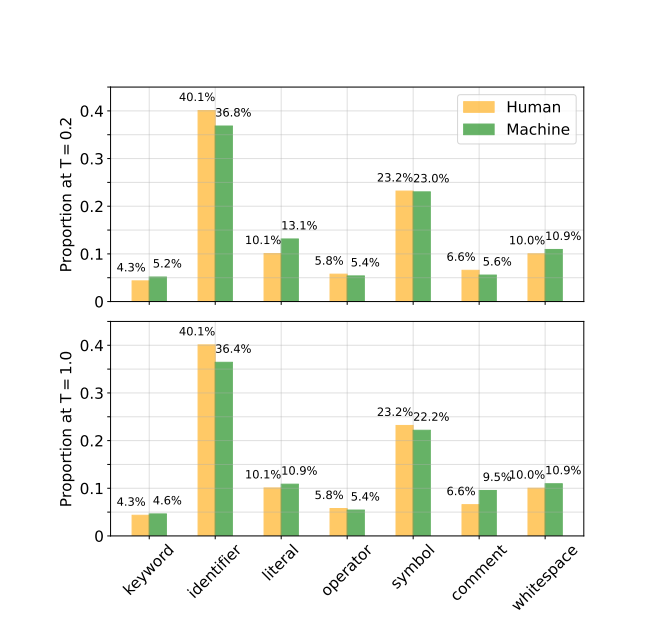
\includegraphics[width=0.95\linewidth]{figs/fig1_syntax_distribution.png}
  \caption{Syntax element distribution of the code corpus, by token category and temperature.}
  \label{fig:syntax-dist}
\end{figure}

\begin{quote}
\textit{Finding 2.} Machine-authored code tends to use fewer identifiers and more literals for direct data processing, and adds more comments as the generation temperature grows.
\end{quote}

\textbf{Zipf's and Heaps' laws.} Both corpora broadly obey Zipf's law -- a small number of tokens dominate usage, with a long tail of rare ones -- and Heaps' law -- vocabulary size grows roughly as a power of corpus length. However, machine-generated code at the low temperature shows a visibly \emph{shallower} Heaps' law slope, meaning its vocabulary grows more slowly as more code is generated, and a stronger concentration of probability mass on tokens ranked between roughly 10 and 100 under Zipf's law. The authors offer three complementary explanations: human variability and creativity naturally spreads token usage more broadly; a model sampled at low temperature is comparatively risk-averse, falling back on familiar, ``safe'' patterns; and some token sequences may simply be over-represented in the training data, biasing the model toward them.

\begin{quote}
\textit{Finding 3.} Machines prefer a narrower spectrum of frequently used tokens, while human code shows richer diversity in token selection.
\end{quote}

\textbf{Conciseness.} At $T=0.2$, machine-generated functions are shorter than their human-written counterparts in both token and line count. This gap narrows considerably at $T=1.0$, though machine code remains somewhat more concise on average. A plausible reading is that concise solutions were more common, or implicitly rewarded, during pretraining, whereas a human developer typically balances several competing goals -- readability, anticipated future edits, comments for other developers -- that tend to make code longer.

\begin{quote}
\textit{Finding 4.} Machine-authored code is more concise, especially at low temperature, while human-authored code tends to be longer, reflecting individual stylistic habits.
\end{quote}

\textbf{Naturalness.} This is the result the whole detection method hinges on. Figure~\ref{fig:naturalness} shows that machine-generated code has systematically higher log-likelihood and lower log-rank than human code -- i.e., it is more ``natural'' under the model, mirroring what has previously been observed for natural-language text. Table~\ref{tab:naturalness} breaks this naturalness gap down by token category. Every category shows a statistically significant gap ($p<0.001$), but \emph{whitespace} stands out with the single largest gap of any category in both log-likelihood and log-rank -- larger even than the aggregate gap over all tokens combined.

\begin{figure}[t]
  \centering
  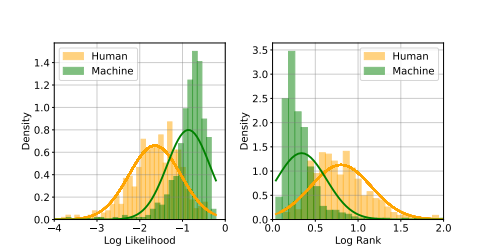
\includegraphics[width=0.95\linewidth]{figs/fig4_naturalness.png}
  \caption{Distribution of naturalness scores (log likelihood, left; log rank, right) for human- vs.\ machine-authored code at $T=0.2$.}
  \label{fig:naturalness}
\end{figure}

\begin{table}[t]
\caption{Naturalness of different syntax-element categories at $T=0.2$; all differences are significant at $p<0.001$.}
\label{tab:naturalness}
\begin{tabular}{@{}lrrrrrr@{}}
\toprule
 & \multicolumn{3}{c}{Log Likelihood} & \multicolumn{3}{c}{Log Rank} \\
\cmidrule(lr){2-4} \cmidrule(lr){5-7}
\textbf{Category} & Mach. & Hum. & $\Delta$ & Mach. & Hum. & $\Delta$ \\
\midrule
keyword    & $-1.701$ & $-2.128$ & 0.428 & 0.837 & 1.053 & 0.217 \\
identifier & $-0.459$ & $-0.874$ & 0.415 & 0.163 & 0.378 & 0.215 \\
literal    & $-0.506$ & $-1.364$ & 0.858 & 0.152 & 0.630 & 0.479 \\
operator   & $-0.938$ & $-1.835$ & 0.897 & 0.367 & 0.872 & 0.504 \\
symbol     & $-0.868$ & $-1.639$ & 0.771 & 0.321 & 0.781 & 0.460 \\
comment    & $-1.503$ & $-3.028$ & 1.525 & 0.608 & 1.610 & 1.002 \\
\textbf{whitespace} & $\mathbf{-1.131}$ & $\mathbf{-2.740}$ & $\mathbf{1.609}$ & $\mathbf{0.429}$ & $\mathbf{1.441}$ & $\mathbf{1.012}$ \\
\midrule
ALL        & $-0.827$ & $-1.658$ & 0.831 & 0.319 & 0.811 & 0.492 \\
\bottomrule
\end{tabular}
\end{table}

This is the empirical justification for DetectCodeGPT's whole design: if whitespace usage is where machine and human code differ \emph{most}, then a perturbation strategy that specifically targets whitespace should be a particularly sensitive probe of authorship.

\begin{quote}
\textit{Finding 5.} Machine-authored code is more ``natural'' than human-authored code overall, and this gap is most pronounced in tokens -- comments and whitespace -- that most directly reflect an individual's personal coding style.
\end{quote}

\subsection{Detection Performance}
\label{sec:detection-perf}
DetectCodeGPT is evaluated on held-out splits of CodeSearchNet and The Stack~\cite{kocetkov2022stack}, against six code LLMs (Incoder, Phi-1, StarCoder~\cite{li2023starcoder}, WizardCoder~\cite{luo2023wizardcoder}, CodeGen2, and Code Llama), at both temperatures, for 24 dataset/model/temperature combinations in total, using AUROC as the metric. Table~\ref{tab:avgauroc} outlines the average AUROC across all 24 dataset/model/temperature combinations for every baseline. DetectCodeGPT achieves the highest average AUROC, showing a $7.6\%$ average relative improvement over the strongest baseline, Log Rank, with the gap confirmed statistically significant by a Wilcoxon rank-sum test ($p<0.001$) over 10 repeated runs. DetectCodeGPT is reported as the single best method in 20 of the 24 combinations. Notably, it also beats GPTSniffer, the \emph{supervised} baseline, on average, despite using no labeled training data at all.

\begin{table}[t]
\caption{Average AUROC across all 24 dataset/model/temperature combinations.}
\label{tab:avgauroc}
\begin{tabular}{@{}lc@{}}
\toprule
\textbf{Method} & \textbf{Avg.\ AUROC} \\
\midrule
Entropy                        & 0.3961 \\
DetectGPT                      & 0.6357 \\
GPTSniffer (supervised)        & 0.6507 \\
LRR                             & 0.7050 \\
NPR                              & 0.7178 \\
Rank                            & 0.7228 \\
Log $p(x)$                      & 0.7649 \\
Log Rank                        & 0.7724 \\
\textbf{DetectCodeGPT (ours)}   & \textbf{0.8308} \\
\bottomrule
\end{tabular}
\end{table}

To see how this plays out per model rather than only on average, Table~\ref{tab:csn02} highlights a slice of the full results table: performance on CodeSearchNet at $T=0.2$, comparing DetectCodeGPT against the two strongest single-statistic baselines. The improvement is consistent across model sizes and families, and is largest for CodeGen2, where DetectCodeGPT gains more than 15 points of AUROC over Log Rank -- the paper attributes CodeGen2's difficulty for other methods to it being trained on a larger share of natural-language text alongside code, which likely blurs its own notion of code ``naturalness.''

\begin{table}[t]
\caption{AUROC on CodeSearchNet ($T=0.2$): representative baselines vs.\ DetectCodeGPT.}
\label{tab:csn02}
\begin{tabular}{@{}lccc@{}}
\toprule
\textbf{Code LLM} & \textbf{Log Rank} & \textbf{NPR} & \textbf{DetectCodeGPT} \\
\midrule
Incoder (1.3B)     & 0.9892 & 0.8143 & \textbf{0.9896} \\
Phi-1 (1.3B)       & 0.7513 & 0.7566 & \textbf{0.8287} \\
StarCoder (3B)     & 0.9340 & 0.9015 & \textbf{0.9438} \\
WizardCoder (3B)   & 0.9120 & 0.8677 & \textbf{0.9345} \\
CodeGen2 (3.7B)    & 0.7199 & 0.6177 & \textbf{0.8802} \\
Code Llama (7B)    & 0.9016 & 0.5890 & \textbf{0.9095} \\
\bottomrule
\end{tabular}
\end{table}

Across the board, detection is markedly harder at $T=1.0$ than at $T=0.2$: higher-temperature sampling makes machine-generated code more diverse and thus more human-like along exactly the dimensions the empirical study measured, which shrinks the naturalness gap the detector relies on. DetectCodeGPT still leads at $T=1.0$, but by a smaller margin.

\subsection{Ablation and Sensitivity Analysis}
Two ablations isolate why DetectCodeGPT works. Table~\ref{tab:ablation} compares the two stylized perturbations, individually and combined, against the traditional masked-language-model (MLM) perturbation used by DetectGPT and DetectLLM. Both newline and space insertion alone already beat the MLM-based perturbation by a wide margin, and combining them performs best at both temperatures -- direct evidence that the earlier empirical finding (whitespace carries the most authorship signal) translates into a better detector, and that avoiding an external rewriting model helps rather than hurts.

\begin{table}[t]
\caption{Ablation of perturbation strategies (Code Llama-7B, The Stack).}
\label{tab:ablation}
\begin{tabular}{@{}lcccc@{}}
\toprule
\textbf{Temp.} & \textbf{MLM} & \textbf{Newline} & \textbf{Space} & \textbf{Newline\&Space} \\
\midrule
$T=0.2$ & 0.5436 & 0.8703 & 0.8639 & \textbf{0.8852} \\
$T=1.0$ & 0.6226 & 0.6453 & 0.6504 & \textbf{0.6660} \\
\bottomrule
\end{tabular}
\end{table}

Table~\ref{tab:perturbcount} sweeps the number of perturbations $k$ used per snippet. AUROC rises sharply from $k=10$ to $k=20$ and then plateaus, with negligible gains beyond $k=50$. This is a practically useful result: it means DetectCodeGPT does not need hundreds of perturbations (and therefore hundreds of extra forward passes) to work well, which keeps it cheap even without an external perturbation model.

\begin{table}[t]
\caption{Effect of the number of perturbations $k$ on AUROC.}
\label{tab:perturbcount}
\begin{tabular}{@{}lccccc@{}}
\toprule
$k$ & 10 & 20 & 50 & 100 & 200 \\
\midrule
$T=0.2$ & 0.6537 & 0.8825 & 0.8852 & \textbf{0.8855} & 0.8846 \\
$T=1.0$ & 0.5558 & 0.6584 & 0.6660 & 0.6660 & \textbf{0.6662} \\
\bottomrule
\end{tabular}
\end{table}

\subsection{Cross-Model Robustness}
A realistic deployment scenario rarely has white-box access to the exact model that generated a suspect snippet. Figure~\ref{fig:crossmodel} illustrates the cross-model experiment, where a \emph{different} LLM is used as the surrogate scoring model $p_\theta$ than the one that actually generated the code. Performance drops only modestly outside the diagonal (white-box) entries: for instance, using StarCoder as the surrogate to detect code from WizardCoder or Code Llama achieves 0.92 and 0.87 AUROC respectively, versus 0.93 for StarCoder detecting its own output. CodeGen2 is the hardest source model to detect in the black-box setting, again plausibly because of its more NL-heavy training mix, though Phi-1 does comparatively well as a surrogate for it (0.83 AUROC), hinting that ensembling several surrogate detectors could help further.

\begin{figure}[t]
  \centering
  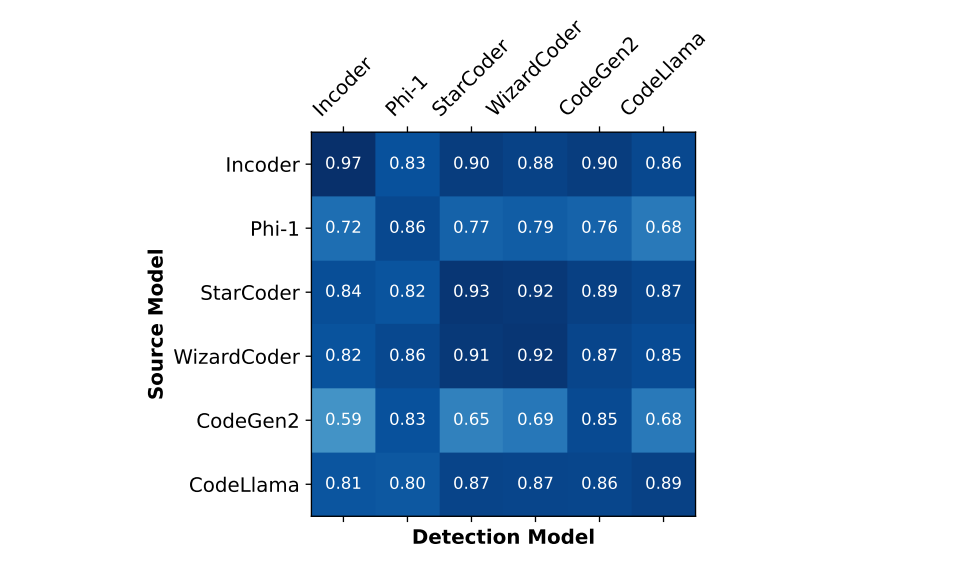
\includegraphics[width=0.85\linewidth]{figs/fig6_crossmodel.png}
  \caption{Cross-model detection performance on The Stack at $T=0.2$: rows are the source (generating) model, columns are the surrogate (detecting) model.}
  \label{fig:crossmodel}
\end{figure}

\subsection{Qualitative Examples}
Figure~\ref{fig:examples} walks through representative snippets and shows, qualitatively, what the quantitative results above mean in practice. In the machine-generated example, DetectCodeGPT correctly flags a snippet where related \texttt{if} statements are grouped together and separated from unrelated code by newlines -- a modular, regularized layout its stylized perturbation is sensitive to. In two human-written examples, both baselines misclassify code that uses whitespace inconsistently (blank lines in some places but not others, or spaces added around some operators but not others), while DetectCodeGPT correctly identifies the irregularity as a human signature. The figure also includes a genuine failure case: a human-written snippet that happens to be unusually well-formatted is misclassified as machine-generated by every method, including DetectCodeGPT, underscoring that consistently tidy human code remains a hard case for this family of detectors.

\begin{figure}[t]
  \centering
  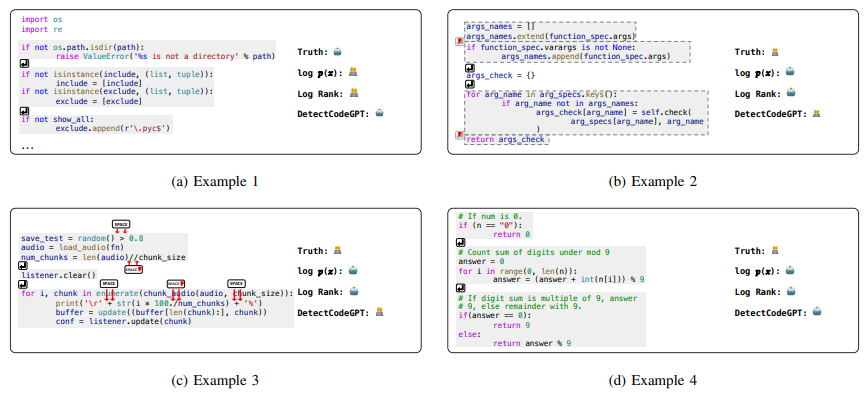
\includegraphics[width=0.95\linewidth]{figs/fig5_examples.png}
  \caption{Representative machine- and human-authored snippets with predictions from Log~$p(x)$, Log~Rank, and DetectCodeGPT.}
  \label{fig:examples}
\end{figure}

\section{Discussion}
\label{sec:discussion}

\subsection{Why DetectCodeGPT Works}
The paper attributes DetectCodeGPT's advantage over prior perturbation-based detectors to two factors, both of which follow naturally from the empirical study in Section~\ref{sec:results}. First, \emph{correctness preservation}: because its perturbations only insert whitespace, they cannot silently break the syntax of the snippet the way masking-and-refilling a token can. An MLM-based perturbation occasionally substitutes the wrong identifier or introduces a type error, and that kind of accidental corruption lowers the naturalness score for reasons that have nothing to do with whether the original snippet was human- or machine-written -- adding noise exactly where the signal needs to be cleanest. Second, \emph{fidelity to how humans actually vary their whitespace}: because Finding 5 shows whitespace is where the naturalness gap is largest, and because human whitespace usage is genuinely closer to random than a model's, sampling insertion counts from a Poisson distribution at randomly chosen locations mimics that human irregularity more faithfully than any single deterministic rule could.

\subsection{Strengths}
Relative to prior perturbation-based detectors, DetectCodeGPT does not need to query an external model to generate its perturbations, which removes both a source of latency and a second point of failure (what if that external model is unavailable, or itself biased in some way?). Relative to supervised detectors like GPTSniffer, it needs no labeled training data at all, and Section~\ref{sec:results} shows it generalizes reasonably well even when the exact source model is unknown -- a property a supervised classifier trained on one family of models cannot easily claim.

\subsection{Limitations and Future Directions}
The study explicitly mentions a few limitations. Computationally, their study is restricted to models of at most 7B parameters, so it remains unclear whether the same lexical, conciseness, and naturalness gaps -- and therefore the same detector -- hold up for today's much larger frontier models. Scope-wise, the entire empirical study and evaluation is conducted on Python; the authors argue, but do not verify, that the approach should transfer to languages such as C/C++, Java, and JavaScript, on the grounds that inserting whitespace is unlikely to change a program's meaning in those languages either. A further limitation visible in the results themselves is that detection accuracy at high temperature ($T=1.0$) still leaves considerable room for improvement, since more exploratory sampling narrows exactly the naturalness gap the method depends on.

\subsection{Reflection}
The most convincing aspect of this methodology is arguably not just the final AUROC numbers, but the core diagnosis in Table~\ref{tab:naturalness} that motivates them: showing \emph{specifically} that whitespace carries the largest naturalness gap of any token category turns DetectCodeGPT from an arbitrary design choice into a directly evidence-driven one. That said, the same diagnosis suggests a fairly obvious limitation the paper does not evaluate directly: if whitespace and formatting are the primary signal, a detector like this one is likely vulnerable to a user who simply runs a generated file through an autoformatter (e.g., \texttt{black} for Python) before sharing it, since that would erase exactly the irregularities the method is built to notice. Testing robustness to routine code formatting -- something a developer might do for entirely benign reasons -- seems like a natural next experiment, and a meaningful complement to the cross-model robustness study already in Section~\ref{sec:results}.

In summary, this study makes two primary contributions worth noting: a careful empirical account of how machine- and human-written code actually differ, and a lightweight detector, DetectCodeGPT, that turns the most discriminative part of that account -- whitespace naturalness -- into a practical, zero-shot, model-agnostic tool for judging code provenance.


\bibliographystyle{ACM-Reference-Format}
\bibliography{references}

\end{document}